\documentclass[a4paper,10pt]{article}

\usepackage[utf8]{inputenc}
\usepackage[T1]{fontenc}
\usepackage[english]{babel}

\usepackage{color}
\usepackage{float}
\usepackage{caption}
\usepackage{subcaption}
\usepackage{fancyvrb}

\usepackage{amssymb}
\usepackage{amsmath}
\usepackage{listings}

\usepackage{graphicx}
\DeclareGraphicsExtensions{.png}

\newcommand{\N}{\mathbb{N}}
\newcommand{\R}{\mathbb{R}}
\newcommand{\Z}{\mathbb{Z}}

\title{DM535 eksamenssæt -- jan2013 \\ \rule{10cm}{0.5mm}}
\author{Studiegruppe F \\ Section S7 \\
DM535\\\rule{5.5cm}{0.5mm}\\}
\date{\today}

\begin{document}
\maketitle
\vfill
\tableofcontents
\newpage
\section{Opgave 1}
\begin{figure}[h]
\center
\caption{Venn diagrammet til opgaven}
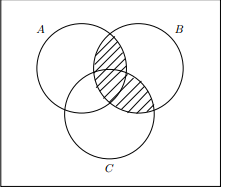
\includegraphics[scale=0.5]{venn-jan13}
\end{figure}
\subsection{a}
\begin{description}
    \item $(A \cap B) \cup (B \cap C)$ \hfill \\
        Som man kan se på diagrammet for oven er den skraverede del altså
        foreningsmængden af fællesmængderne for henholdsvis $A$ og $B$ og $B$
        og $C$. Denne svarer derfor til diagrammet.
    \item $(\overline{A \cup B}) \cap C$ \hfill \\
        Denne passer \textbf{ikke} til venn-diagrammet, da dette er ækvivalent
        med $ (C - B) - A$.
    \item $B - (\overline{A \cup C})$ \hfill \\
        Denne mængde er som venn diagrammet nedenunder og repræsenterer derfor
        \textbf{ikke} venn diagrammet for oven.
        \begin{figure}[h]
        \center
        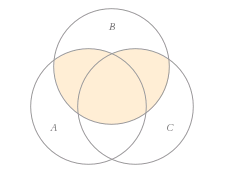
\includegraphics[scale=0.5]{venn2-jan13}
        \end{figure}
    \item $(A \cup C) \cap B$ \hfill \\
        Denne mængde passer til opgavens venn-diagram da den er ækvivalent med
        udsagnet $(A \cap B) \cup (B \cap C)$ grundet ``Distributive Law''(s.
        132 i bogen).
\end{description}

\subsection{b}
Da $A$ er tælleligt uendelig, og $B$ er endelig(og derfor tællelig), er
kardinaliteten af $A \cap B$ også tællelig. Mere kan vi ikke sige.

\section{Opgave 2}
\[ 
    A = \{2, 4, 8, 16\}
\]
Husk at $y|x$ betyder at $y$ går op i $x$ eller $y$ dividerer $x$.
\subsection{a}
\[ 
    \forall x \in A\colon \exists y \in A\colon y|x 
\]
Dette udsagn kan læses som ``for alle $x$ i $A$ findes der et tilsvarende $y$
i $A$ der går op i $x$''. Dette udsagn er \textbf{sandt} da $2$ går op i alle
elementer i $A$.
\subsection{b}
\[ 
    \exists x \in A\colon \forall y \in A\colon y|x 
\]
Dette udsang kan læses som ``der findes et $x$ i $A$ som alle tal i $A$ går op
i''. Dette udsagn er også \textbf{sandt} da alle elementer i $A$ går op i
$16$.
\subsection{c}
\[ 
    \forall x \in A\colon \forall y \in A\colon y|x 
\]
Dette udsang kan læses som ``alle elementer i $A$ går op i alle elementer i
$A$''. Dette udsagn er \textbf{falsk} da f.eks. $16$ ikke går op i $8$. 

\section{Opgave 3}
\[
A = 
\begin{bmatrix}
    2 & 2 \\
    2 & 2 
\end{bmatrix}
\ \ 
B = 
\begin{bmatrix}
    1 & 2 \\
    3 & 4 
\end{bmatrix}
\]

\subsection{a}
\begin{align*}
    A \cdot B &= 
\begin{bmatrix}
    2 & 2 \\
    2 & 2 
\end{bmatrix}
\cdot
\begin{bmatrix}
    1 & 2 \\
    3 & 4 
\end{bmatrix} \\
&= 
\begin{bmatrix}
    8 & 12 \\
    8 & 12 
\end{bmatrix} \\
\end{align*}

\subsection{b}
\[
    C = 
    \begin{bmatrix}
        c_{11} & c_{12} \\
        c_{21} & c_{22} \\
    \end{bmatrix}
\]
Hvor $c_{11}, c_{12}, c_{21}, c_{22} \in \Z$.
Matricen $A \cdot C$ vil derfor se sådan ud:
\[
    A \cdot C = 
    \begin{bmatrix}
        2 & 2 \\
        2 & 2 
    \end{bmatrix}
    \cdot
    \begin{bmatrix}
        c_{11} & c_{12} \\
        c_{21} & c_{22} \\
    \end{bmatrix}
    =
    \begin{bmatrix}
        2c_{11} + 2c_{21} & 2c_{12} + 2c_{22} \\
        2c_{11} + 2c_{21} & 2c_{12} + 2c_{22} \\
    \end{bmatrix}
\]
Lad os se på tallet $2c_{xy} + 2c_{xy}$, hvor $x, y \in [1,2]$. 
Da $2$ er et heltal, og $c_{xy}$ er et heltal, vil tallet $2c_{xy}$ også være
et heltal per definition. Derfor vil summen $2c_{xy} + 2c_{xy}$ også være et
heltal per definition da det er en sum af to heltal.

\section{Opgave 4}
\subsection{a}
\begin{align*}
    x \equiv 1 \pmod 2 & \qquad (1) \\
    x \equiv 2 \pmod 4 & \qquad (2)
\end{align*}
Dette kongruens-system har ingen løsninger. Kongruens 1 har kun løsninger i de
ulige tal, mens kongruens 2 har løsningerne $2 + 4k$ hvor $k \in \Z$, som er
lige tal.

\subsection{b og c}
Vi skal løse kongruens-systemet 
\begin{align*}
    x \equiv 1 \pmod 2 & \qquad \\  
    x \equiv 2 \pmod 3 & \qquad \\  
    x \equiv 3 \pmod 5 & \qquad 
\end{align*}
Vi kan løse dette kongruens-system ved brug af den Kinesiske
Restklassesætning, da $2, 3, 5$ er alle parvist indbyrdes primiske. Altså hvis
man vælger to tal ud af de tre tal er største fælles divisor af de tal altid
1.

For at løse dette ved brug af den kinesiske restklassesætning starter vi med
at udregne $m$ og opstiller defter alle $a_k, m_k, M_k$ for $k \in
\{1,2,3\}$. $m = 2 \cdot 3 \cdot 5 = 30$.
\begin{align*}
\begin{matrix}
    a_1 = 1 & m_1 = 2 & M_1 = \frac{m}{m_1} = 15 \\
    a_2 = 2 & m_1 = 3 & M_2 = \frac{m}{m_2} = 10 \\
    a_3 = 3 & m_1 = 5 & M_3 = \frac{m}{m_3} = 6 \\
\end{matrix}
\end{align*}
Nu skal vi løse tre kongruenser enkeltvis, ved at finde den multiplikative
inverse til hver enkelt.
\begin{align*}
    15y_1 &\equiv 1 \pmod 2 \\
    10y_2 &\equiv 1 \pmod 3 \\
    6y_3  &\equiv 1 \pmod 5 
\end{align*}
Disse er ret simple at løse i dette tilfælde og kan blot løses via
observation, da alle $y$-værdierne er $1$.

Nu er den endelige løsning 
\[
    x = \sum_{k = 1}^{n} M_k y_k a_k
\]
Hvor $n = 3$ i vores tilfælde da vi løser et kongruens-system med 3
kongruenser. 
\begin{align*}
    x &= \sum_{k = 1}^{3} M_k y_k a_k = 
        15 \cdot 1 \cdot 1 + 10 \cdot 1 \cdot 1 + 6 \cdot 1 \cdot 3 \\
    x &= 53
\end{align*}
Det vil sige at $x$ er en løsning, og at der findes én unik løsning til
kongruens-systemet mellem $0$ og $m - 1$. 
Da $53 = 1\cdot 30 + 23$ er $x \equiv 23 \pmod{30}$.

I intervallet $\Z_{89}$ findes der derfor \textbf{tre} løsninger,
nemlig $x = \{23, 53, 83\}$.

\end{document}
